
%(BEGIN_QUESTION)
% Copyright 2014, Tony R. Kuphaldt, released under the Creative Commons Attribution License (v 1.0)
% This means you may do almost anything with this work of mine, so long as you give me proper credit

Denne gruppen stolpemonterte krafttransformatorer transformerer 7.2 kVAC linjespenning ned til 240 VAC for å forsyne en liten bedrift:

$$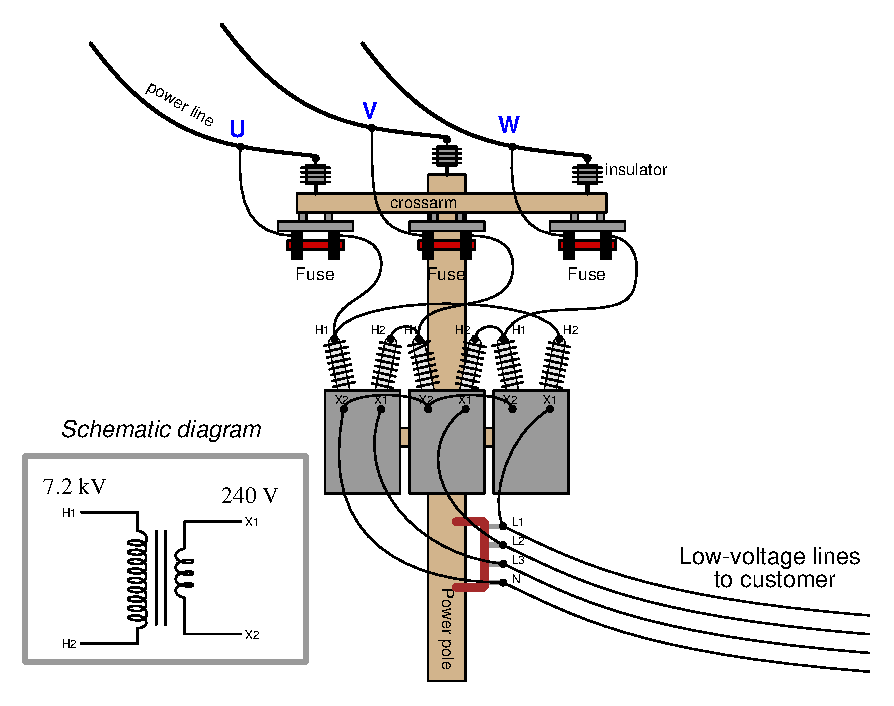
\includegraphics[width=15.5cm]{i00826x01.eps}$$

Gitt følgende linjespenninger (målt fase-mot-jord), beregn fasevinklene for de oppgitte sekundærspenningene:

\begin{itemize}
\item{} $V_U$ = 4160 V $\angle$ $0^o$
\item{} $V_V$ = 4160 V $\angle$ $-120^o$
\item{} $V_W$ = 4160 V $\angle$ $-240^o$
\end{itemize}

\vskip 10pt

\begin{itemize}
\item{} $V_{L1-N}$ = \underbar{\hskip 20pt} $\angle$ \underbar{\hskip 10pt}
\vskip 5pt
\item{} $V_{L2-N}$ = \underbar{\hskip 20pt} $\angle$ \underbar{\hskip 10pt}
\vskip 5pt
\item{} $V_{L3-N}$ = \underbar{\hskip 20pt} $\angle$ \underbar{\hskip 10pt}
\vskip 5pt
\item{} $V_{L1-L3}$ = \underbar{\hskip 20pt} $\angle$ \underbar{\hskip 10pt}
\end{itemize}

\vskip 20pt \vbox{\hrule \hbox{\strut \vrule{} {\bf Forslag til sokratisk diskusjon} \vrule} \hrule}

\begin{itemize}
\item{} Har disse krafttransformatorene {\it additiv} eller {\it subtraktiv} polaritet? Hvordan ser du det?
\item{} Identifiser fasesekvensen (fase{\it rotasjon}) i dette kraftsystemet basert på oppgitte fase-mot-jord-verdier.
\end{itemize}

\underbar{file i00826}
%(END_QUESTION)





%(BEGIN_ANSWER)

\noindent
{\bf Delsvar:}

$$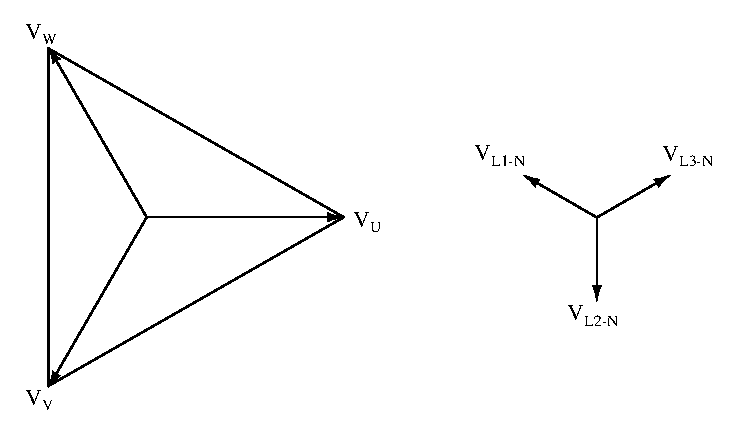
\includegraphics[width=15.5cm]{i00826x02.eps}$$

%(END_ANSWER)





%(BEGIN_NOTES)

Når hver transformator får 7200 volt på primærviklingen, vil hver sekundærvikling gi 240 volt. Primærviklingen i venstre transformator får fasoren $V_U - V_V$ med retning +30$^{o}$, så $V_{L3}$ får samme vinkel. Primærviklingen i midterste transformator får fasoren $V_V - V_W$ med retning $-90^o$, så $V_{L2}$ får samme vinkel. Primærviklingen i høyre transformator får fasoren $V_W - V_U$ med retning $150^o$, så $V_{L1}$ får samme vinkel.

\begin{itemize}
\item{} $V_{L1-N}$ = 240 V $\angle$ $150^o$
\vskip 5pt
\item{} $V_{L2-N}$ = 240 V $\angle$ $-90^o$
\vskip 5pt
\item{} $V_{L3-N}$ = 240 V $\angle$ $30^o$
\vskip 5pt
\item{} $V_{L1-L3}$ = 415.7 V $\angle$ $0^o$
\end{itemize}

Merk at fasefølgen på primærsiden er {\it UVW}, mens fasefølgen på sekundærsiden er {\it 321}.

%INDEX% Electronics review: AC transformer circuit
%INDEX% Electronics review, phasor expressions of circuit quantities
%INDEX% Electronics review, 3-phase transformer bank phase shift calculations

%(END_NOTES)
